\paragraph{Motivation}

Physics in general and particle physics in particular is buinding unprecedented high resoultuion and high speed detectors. 
Due to the increase of the number of detector channels and the high rate of their readout, the data volume that will be produced by experiments is one of two orders of magnitude bigger compared to the sizes we are used nowadays. The tecnology to deal with such a high data volume is either not available yet or at a price tag not accessible by experimental collaborations e.g. present at LHC. It is important to mention that high data volume has direct implication on the Data Acquisition Systems (DAQs), on the Trasfer Systems and on the long term Storage Systems. Data analysis of big data volumes becomes exponentilly complicated as function of the data size itself. The scientific community is investing a significant effort in reducing the experiment data volumes using two parallel approaches, a highly selective, but still cohmprensive event selection (e.g. online trigger) or a data compression trough high performance data compression algorithms. 
As of today, online triggering is still limited to performance of the reconstruction algorithms requiring a significant amount of CPU time. As a consequence only a primarely selection can be achieved with nowadays triggering techniques. 

The compression algorithm used up to now in particle physics experiment are lossless so allowing only a limited compression factor. Higher compression level may be achieved using lossy comoression techniques. However, the tuning of the lossy algorithm need to be tailored to the user case and validated against the data analysis physics goal of the dataset collected. This approach is extremely expensive in term of personapower with very slow turnaround cycles. A RAW data event produced by a detector is in general composed by a collection of RAW data produced by the sub-detectors composing the experiment. Each of the sub-detectors in general has a unique data type so in order to achieve the highest compression factor, each sub-detector data type needs to be treated indipendently with hits specific compression algorithm or tuning. It is also important to bare in mind that the RAW data tier is only the first tier used in a data analysis process. The RAW data are usually processed creating general Analysis Object Data (AOD). The AOD are then processed again to create the smaller AOD versions and targeted to specific data analysis. The multi-tier approach is essential to reduce to its minimum the needs of data processing but it has a negative effect on the toal amount of storage required. In orger to get efficine data reduction, each data-tiers must be compressed with a dedicated compression algorithm specifically tuned for the purpose.  As a consequence of what descrived above, an efficient definition/tuning of a lossy compression strategy has an extremely high number of variables making the approach extremely expensive in term of personpower.

We propose to develop a different approach to this techqnique creating a Machine Learning (ML) based framework trained on data and/or MC, able to identify the most efficient algorithms and tunings preseving the data fidelity for the physics analysis purpose/s. This framework, which employs a Deep Neural Network (DNN) and the recently developed Generative Adversarial Networks (GAN) will learn the requirements of the final physics object (e.g. resolution, systematic error, etc.) and will select the best set of algorithms for the task as well as the settings to be used.

Data reduction trough event selection either online or offline is a crucial aspect on the overall challange. As of today, trigger algorithms reconstrcut partilly the data and extract a subset of the physics observable that should be used for data analysis. While this approach gurantees data fidelity, it is too CPU demanding in particular in the optic of always increasing data rates(FIXME: add here references to sPHENIX and HL-LHC). We propose to develop a different approach using a ML framework including immagine recogniztion tecqniques. The RAW data produced by a detector may indeed be seen as an image from where the phsyics objects may be identified without the needs of their full riconstruction. A ANN and/or a GAN may be trained using data or MC containing the specific object of interest (FIXME: maybe mention proposal 2493). 
 

   




a novel lossy universal compression algorithm embedded in an AI framework with tools such as variational autoencoders that allows autonomous control and optimization of both compression ratio and fidelity for peta-scale data sets



\line(1, 0){15 cm}

\line(1, 0){15 cm}

\line(1, 0){15 cm}

OLD TEXT

Analyses of large physics data sets typically rely on extensive Monte Carlo (MC) simulations that aim to describe the underlying physical processes, backgrounds, and detector response. We propose to develop an entirely different  approach, augmenting or replacing the traditional role of MC , will allow to generate MC samples that reproduce detector data entirely. The GAN and DNN based algorithms will be also used to perform transformation of the data point-cloud to a "truth level" point-cloud, with the ultimate goal of dissecting the data down to its basic information content in terms of known and novel physics particles and processes, opening an era of ML-based discovery physics.

Prototypical examples of the current use of MC simulations are found in high-energy and nuclear physics, for both elementary proton-proton (\pp) or electron-electron (\eecol) collisions systems, and for the complex collisions involving atomic nuclei (\eA, \pA, or \aacol). Here, simulations are needed to model background contributions, their sources, and to determine the response matrix of detectors. Simulation are used also to separate signal and background particles, extracting parameters like efficiency, resolution, and purity. This information obtained from MC simulations enables the interpretation of  measurements in real data. However, knowledge and models for the sum of all physics phenomena observed in data are typically incomplete, and no MC simulation can perfectly reproduce all physics processes. Simulations are continually updated through the release of new ``tunes'', as more precise understanding develops. The complexity of one {\aacol} collisions (which can produce orders of magnitude more particles than one \eecol/{\pp} collision) also means that to-date, the richness of the underlying physics is much less well understood than for \eecol/{\pp}, making the MC tuning much less reliable. This is a major challenge for present and future experimental programs at the CERN Large Hadron Collider (LHC) and the RHIC and EIC facilities at Brookhaven National Laboratory.

Reliable MC modeling requires consideration of time-dependent variations in detector conditions and response, such as alignment between detectors, calibrations and detector aging. This often leads to the introduction of additional `residual' corrections in the analysis process, accounting for aspects not understood in simulations. As a consequence the physics results carry additional uncertainties, diluting the power of interpretation and new physics knowledge they carry. High-accuracy/sensitivity and in general any discovery studies (\eg, Higgs or neutrino measurements) are extremely sensitive to the reliability of the MC modeling.

Whether looking at signal or background in MC simulations, an additional factor is the statistical precision of the MC studies, which should be commensurate with that of the collected experimental data. Taking LHC as example, this leads to the additional challenge that improvements in accelerator performance and data collection require increasingly large data samples, far outpacing the increase in available computing resources (CPU and storage) for simulations. This challenge will become more pressing in the future ``high luminosity'' era of LHC operations, requiring resources for MC sample production that cannot be easily met (e.g., an estimated increase from ~40 to ~500PB of disk needs from 2020 to 2030). Availability of workforce and computing resources to address the simulation needs of many concurrent analyses, often involving multiple iterations, is rapidly becoming the major bottleneck in the overall data analysis enterprise. Current mitigation strategies to address high statistics MC sample needs include discarding part of the information content in the simulation process and using so-called fast simulations, in which the detector response is approximated through parametrizations. Such  strategies inevitably lead to less overall accuracy. 
\vspace{-0.5cm}
\paragraph{Proposal} Our plan has three main objectives as illustrated in the flow-chart in Fig.~\ref{fig:concept} (left):

\textit{Data to ML:} To reproduce most accurately the collision environment (background, signal, and run conditions), we plan to develop a GAN algorithm fed by real data and capable of separating/tagging background samples from signal samples in the data itself.

\textit{MC to ML:} To shorten the simulation time, the GAN/DNN framework will replace the `person made' and imperfect description of the detector response included in fast simulation through an automatic, data-driven generation of relevant parametrizations.

\textit{Data to MC:} To uncover known and unknown physics processes in data, the GAN/DNN framework will be fed real events and tasked to disassemble them into basic sets of constituents, allowing a `particle level' analysis close to the one possible at ``truth'' level in MC events. Importantly, this approach will make it possible to continue analysis of archived data  from completed experiments, for which no new simulations are available.

%We note that our problem is not a simple data processing problem. By using real data, physics input, we add additional constrain and break/prevent the degeneracy of the algorithm. 

\begin{figure}[!ht]
\vspace{-0.4cm}
\begin{center}
\includegraphics[width=.5\textwidth]{}
%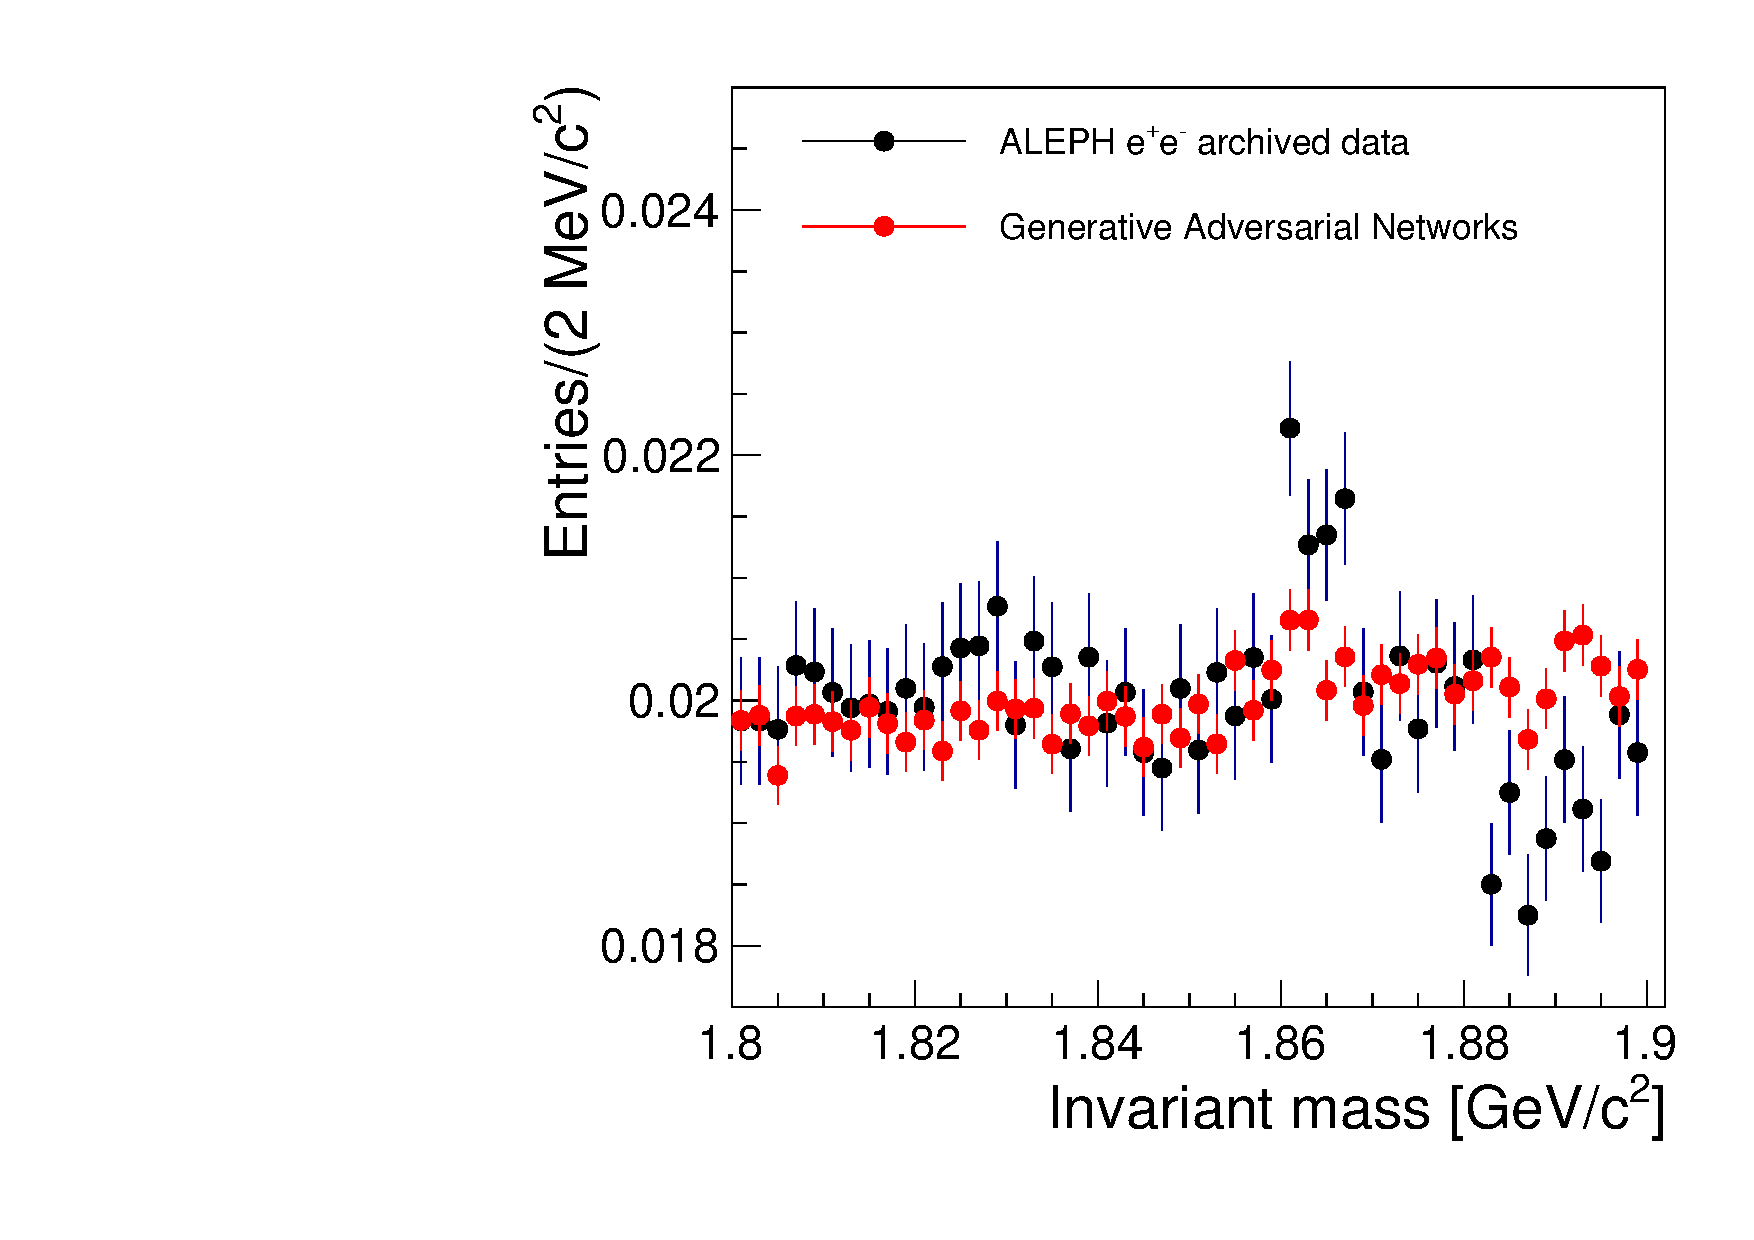
\includegraphics[width=.25\textwidth,keepaspectratio]{outputFig}
\hspace{0.03\textwidth}
\includegraphics[width=.25\textwidth,keepaspectratio]{}
\vspace{-0.5cm}
\caption{}
\label{fig:concept}
\end{center}
\end{figure}
\vspace{-0.8cm}

We have performed feasibility studies for this new approach, evaluating so far one GAN algorithm, tableGan (a convolutional neural network known for its performance and flexibility in representing data), with which we have created first demonstrators using cloud computing resources. These evaluations were performed using {\eecol} archived data from the ALEPH experiment (which ended data taking in 2000), for which the background levels are low, and the theoretical descriptions are more precise. The input and output point-clouds are based on particle momentum vector,  type and charge, as well as event multiplicity. Preliminary results are shown in Fig.~\ref{fig:concept} (right). Importantly this demonstrates that while the input for the tableGAN training was based on single particle observables, the GAN based algorithm could also describe correlated two-particle observables, such as the invariant mass distribution shown. This includes both the bulk (combinatorial) background shape and fine details in the simulation such as the $D^0$ meson resonance peak. In our approach, one could then use the output particles to perform other physics analysis (\eg, reconstruct other mesons decays). While still at an early stage, the ML implementation today is already demonstrating that it could generate {\eecol} events that are similar to real data. Before deciding on the final approach, other algorithms will be evaluated. These will include ctGAN, which was demonstrated to generate synthetic tabular data with high fidelity; $\alpha$-GAN, a hybrid approach combining a likelihood based model (variational auto-encoders, VAEs), and an implicit generative model (GANs) to combine an adversarial loss with a data reconstruction loss; VQ-VAE-2, a vector quantized VAE model, which uses hierarchical multi-scale latent maps for achieving an increased resolution; InterFaceGAN, which interprets the latent semantics learned by GANs for semantic face editing. 

The proposal aims to conduct foundational research to develop reliable and efficient ML tools and approaches to exploit new computational technologies in order to find solutions for one of the most challenging problems in nuclear, particle and neutrino physics, and many areas of high-precision research in general: the size of the MC samples and the accuracy of MC modelling. The proposed research  also aims to profoundly change data analysis, employing graph and network algorithms for discovery: training the machine to uncover yet-unknown physics.
\clearpage


